\documentclass{report}
\usepackage{contour}
\usepackage{ulem}
\usepackage{caption}
\usepackage{subcaption}
\usepackage{geometry}
\geometry{
letterpaper,
left=1in,
right=1in,
bottom=1in,
top=1in,
}

\renewcommand{\ULdepth}{1.5
pt}
\contourlength{0.8pt}

\newcommand{\myuline}[1]{%
  \uline{\phantom{#1}}%
  \llap{\contour{white}{#1}}%
}

\renewcommand{\baselinestretch}{1.5}

\begin{document}

\begin{titlepage}
    \begin{center}
    \vspace*{1cm}

    \textbf{Praxis II - Student Engineering Handbook}

    \vspace{0.5cm}
    \textit{ESC102 Final Assessment}

    \vspace{1.5cm}

    J. Lefebvre\\\small{jayden.lefebvre@mail.utoronto.ca}\\\small{Student Number: 1006861344}

    \vfill

    \vspace{0.8cm}

    Engineering Science\\
    Faculty of Applied Science and Engineering\\
    University of Toronto\\
    Tuesday April 30th, 2021

    \end{center}
\end{titlepage}

\tableofcontents
\pagebreak

\section{Introduction}
The purpose of this handbook is to document my learning and position 
as an engineer and designer at this point in my development. It will 
accomplish this by documenting my design products, and the tools/
models/frameworks I have used to achieve those, as well as reflecting 
on each in terms of their utility to future design work. In addition, 
this handbook documents my personal engineering design process as it 
stands currently.

This handbook is created in the hopes that it will be of some design 
assistance to future me. To navigate this document, refer to the Table 
of Contents.
\section{Position}
My approach to designing is best described as top-down: I consider 
myself a big-picture person, so when confronted with a problem, I am 
often able to see the larger solution before imagining its subcomponents. 
I have found that this is highly dependent on how related the problem 
is to both my existing design work as well as my interests; the closer, 
the more easily I can conceive a solution. In this way, so long as I am 
able to properly frame a problem and break it down into its component 
parameters (more on that in Process), the more easily, reliably, and 
rigorously I am able to diverge and converge on solution features.

Since the way I approach problems is “solution-first”, that often puts 
me in an interesting position when it comes to teamwork. Often during 
the first team meeting after being presented a problem, I will present 
my potential solution, and encourage my team to play with the parameters 
conceptually. While this does accelerate the decision-making process and 
put me in a position of leadership I am comfortable with, this also means 
that some team members might be uncomfortable with sharing ideas non-tangential 
to the initially-proposed solution, reducing the overall scope of diverging. 
In my opinion, this is the ultimate design paradox: the wider the scope, 
the better you can diverge, but the less features and parameters are 
shared between designs, and thus it becomes very difficult to converge 
on one feature set on a detailed level.
\pagebreak
I also have certain biases when it comes to problem-solving. Since I have 
been working with technology (programming, electronics, etc.) creatively 
for most of my life, I am inclined to use it to develop solutions even 
if it means increasing the complexity. My interest in technology is one 
of the main reasons I decided to become an engineer.

One of the most interesting things I’ve learned since coming to EngSci 
last september has been the value of rigor. I’ve learned that despite being 
able to solve a problem, it is just as important to be able to show how 
you got there, and why each decision was made. This is especially true when 
it comes to open-source work, which I am passionate about, as it allows 
people to contribute to projects collaboratively and freely.

Finally, one of the first lectures of Praxis II asked the question: “Do you 
consider yourself as more of an engineering student or a student engineer?” 
This was thought-provoking for me, as although I have been academically 
successful for my entire life, it wasn’t the learning that brought me joy; 
it was instead being able to apply what I’ve learned to a real-world problem 
that interested me. This has led me to focus more on projects, real-world 
problems, design teams, and startups in my first year than I had anticipated:
\begin{itemize}
    \item Electronics Engineer w/ UofT Hyperloop Team, working with sensors, 
    protocols, state machines
    \item Project Lead w/ UofT CloudClub, teaching other eng. students professional 
    web dev. techniques, frameworks, and practices
    \item Founded UofT Agritech, developing an autonomous controlled-environment 
    agriculture solution, going to compete in the NASA/CSA Deep Space Food Challenge
\end{itemize}

\pagebreak
\section{Products}
\subsection{Praxis I Personal Engineering Recommendation}
This was my first attempt at engineering design. Since taking a number of 
research and writing composition courses in highschool, I had become accustomed 
to a certain style of writing. Although this writing style translated well 
into claim-argument form, I failed to meet some of the key targets of engineering 
design, including employing the tools and frameworks provided for comparative 
analysis of design candidates. The assessment of my performance reflected this.

\begin{figure}[h]
    \centering
    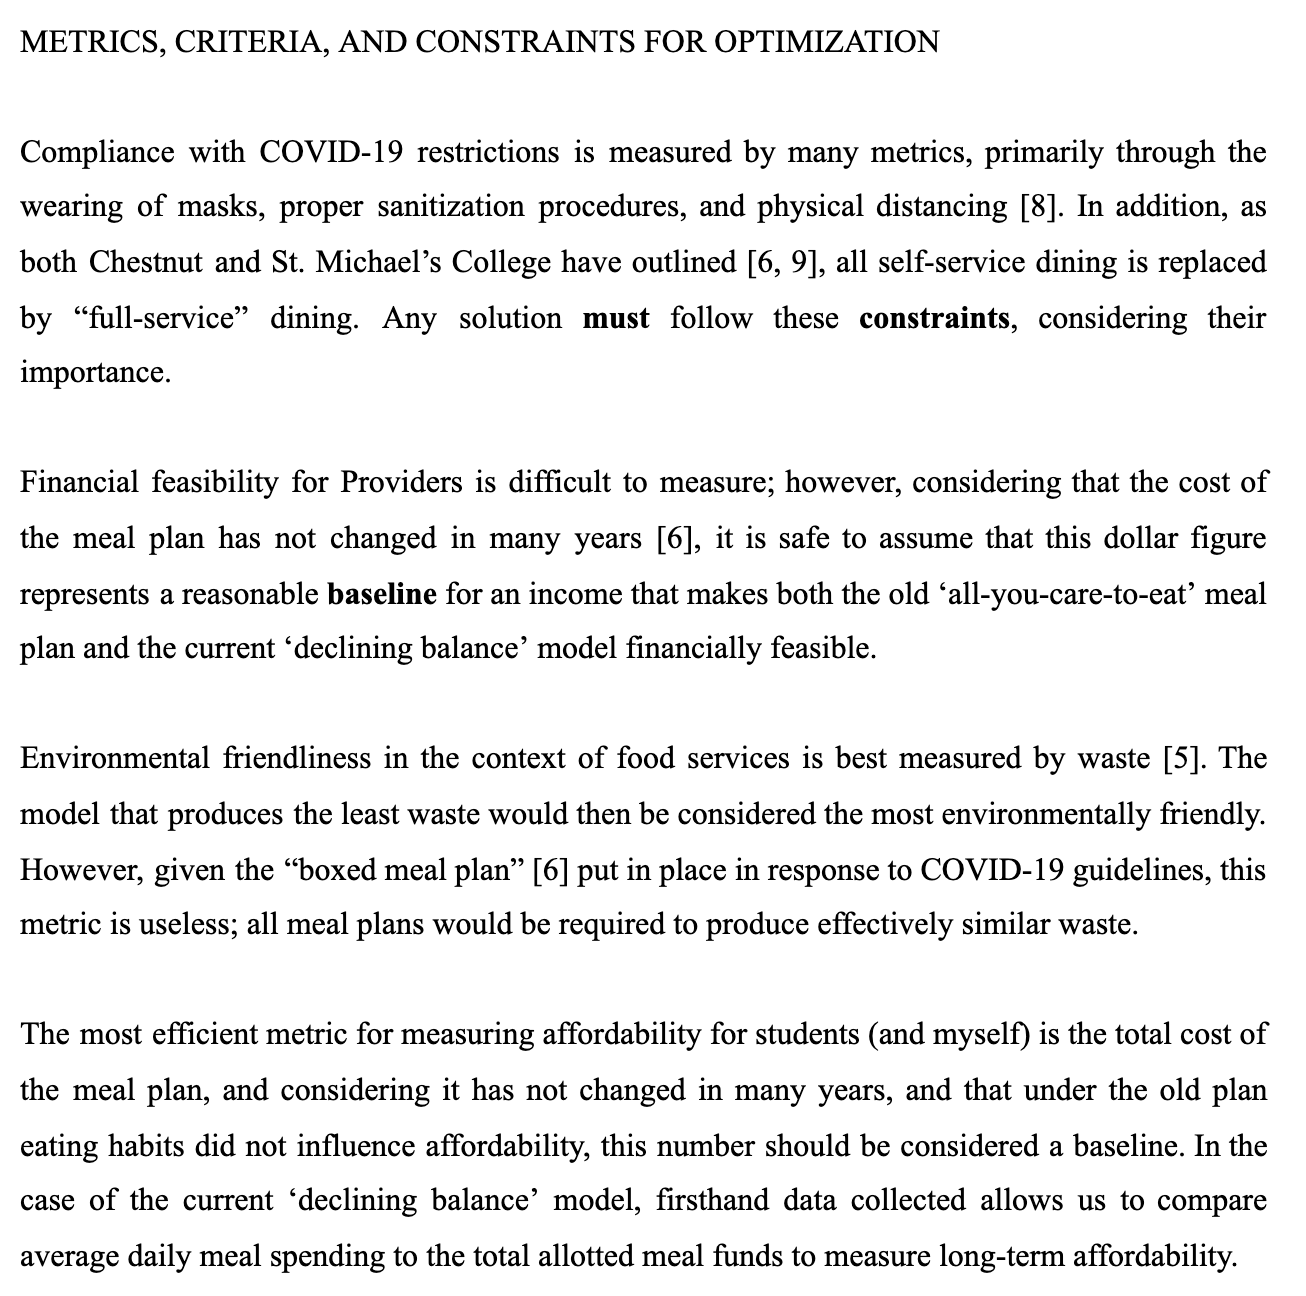
\includegraphics[width=\textwidth/2]{images/per.png}
    \hfill
    \caption{An extract from my PER - note the distinct lack of tables or figures in the metrics section. Odd \cite{per}.}
\end{figure}

\subsection{Praxis I Framing - Design Brief}
This was my second attempt at engineering design, and I took the framing 
failures from the PER and applied new strategies to avoid those pitfalls. 
I had gained a more thorough understanding of the FDCR process. I was also 
able to apply my passions for both plants and technology towards this design 
brief, leading to a greater degree of personal investment, which I believe 
is key to good framing.

% TODO: Framing sprint analysis

\begin{figure}[h]
    \centering
    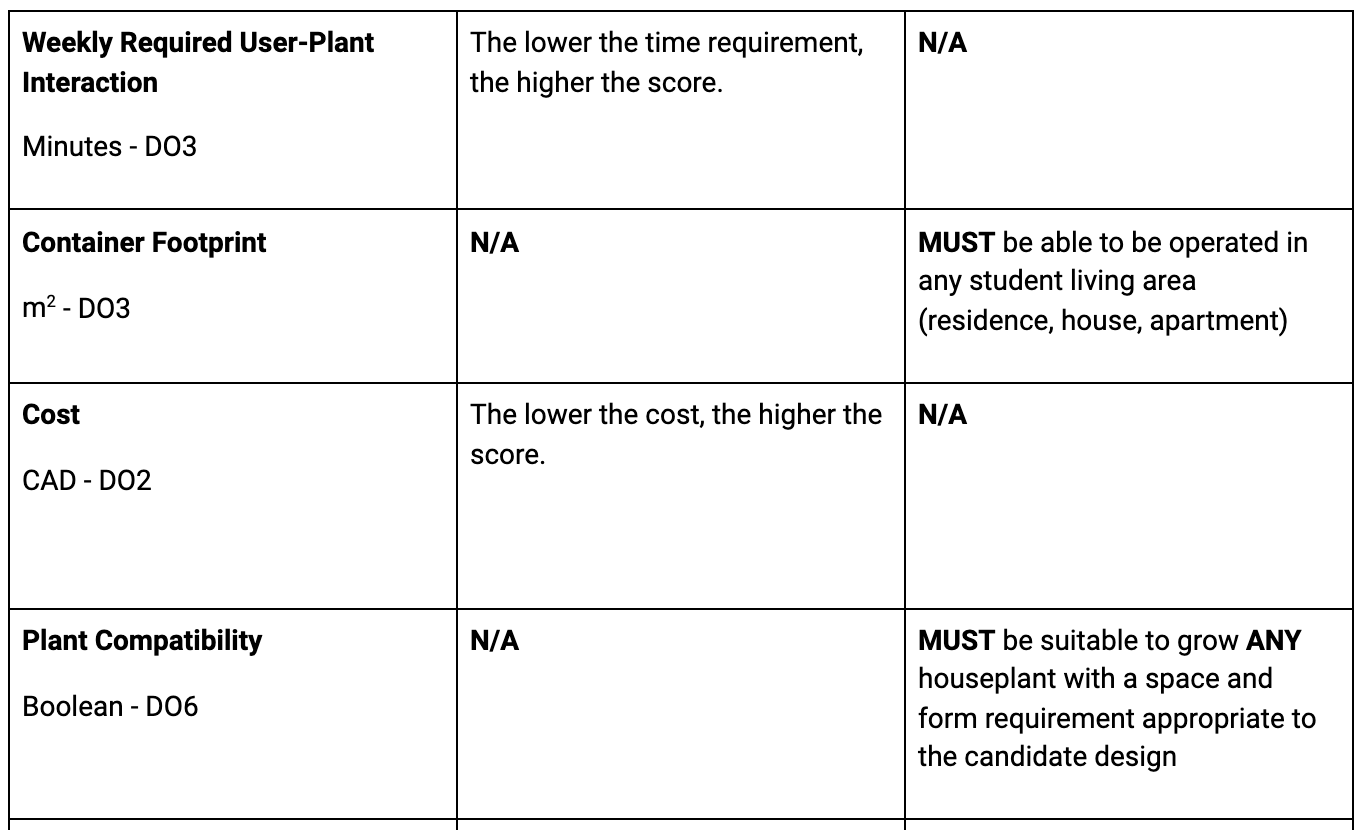
\includegraphics[width=\textwidth/2]{images/designbrief.png}
    \hfill
    \caption{An extract from my framing sprint team's design brief - note the proper use of metrics, with corresponding units, etc. \cite{designbrief}.}
\end{figure}

\subsection{Praxis I Diverging - Candidate Design Parameterization}
During this sprint, I began to form the basis for my personal engineering 
design process. Since the design brief provides both the necessary requirements/
constraints and broken down objectives, it became easy to anchor our diverging 
and establish a list of parameters from those two (respectively). This allowed 
us to use \myuline{attribute listing} and \myuline{reverse brainstorming} to develop a better 
understanding of the parameters, and generate new features based on them.

% TODO: Diverging sprint analysis

\begin{figure}[h]
    \centering
    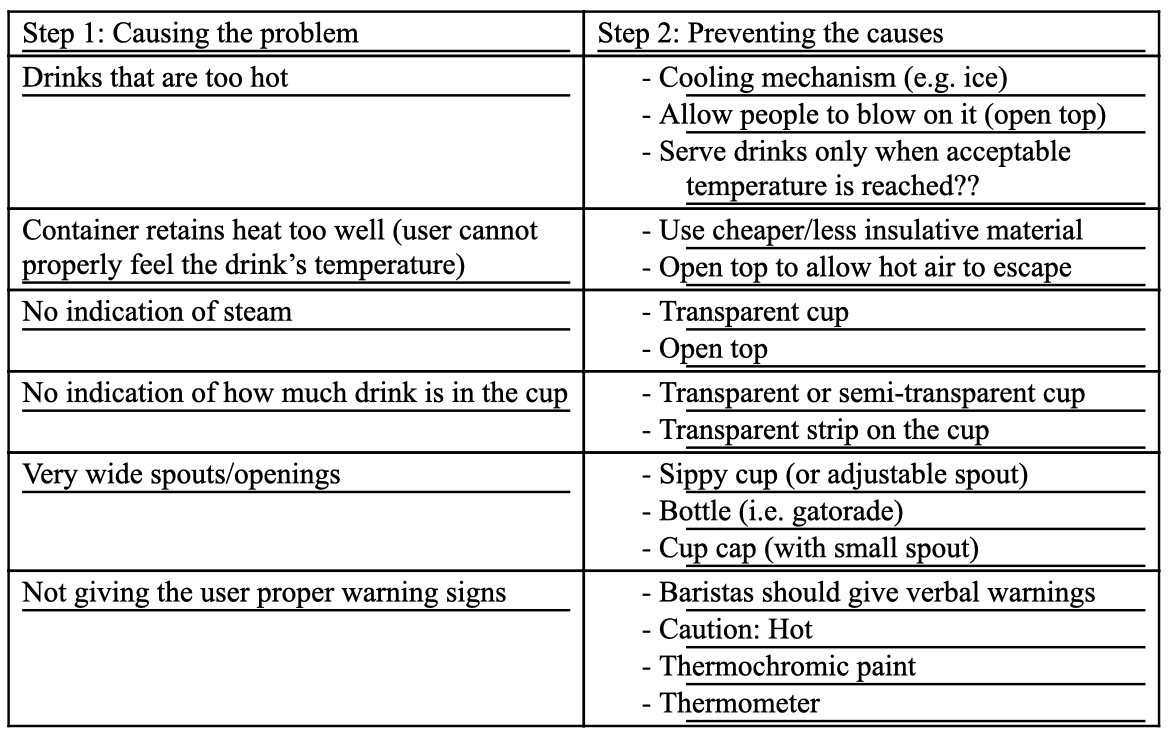
\includegraphics[width=\textwidth/2]{images/parameterization.png}
    \hfill
    \caption{An extract from my diverging sprint team's Candidate Designs and Tools Critique, showing the use of design parameters in the context of \uline{reverse brainstorming} \cite{candidatestools}.}
\end{figure}

\subsection{Praxis I Converging - Design Critique and Categorization}
During the converging sprint, I was able to expand my personal process to 
incorporate diverging in a way that matched the “parameterization” approach 
I had already developed. My converging sprint team found that the candidate 
designs generated during the previous sprint were hard to compare along the 
general metrics of success provided by the design brief. This was due to the 
function differences - each design approached the problem in a radically 
different way. However, there were some that could be grouped together along 
similar functions, and then compared within the category with derived metrics 
appropriate for that category’s function. Once the categories were developed, 
a genetic algorithm was employed, pulling together feature assessment 
(\myuline{Pugh chart}), recombination (\myuline{MORPH chart}), and ultimate category candidate 
prototyping and comparison to develop one singular candidate from a highly 
diverse pool.

\begin{figure}[h]
    \centering
    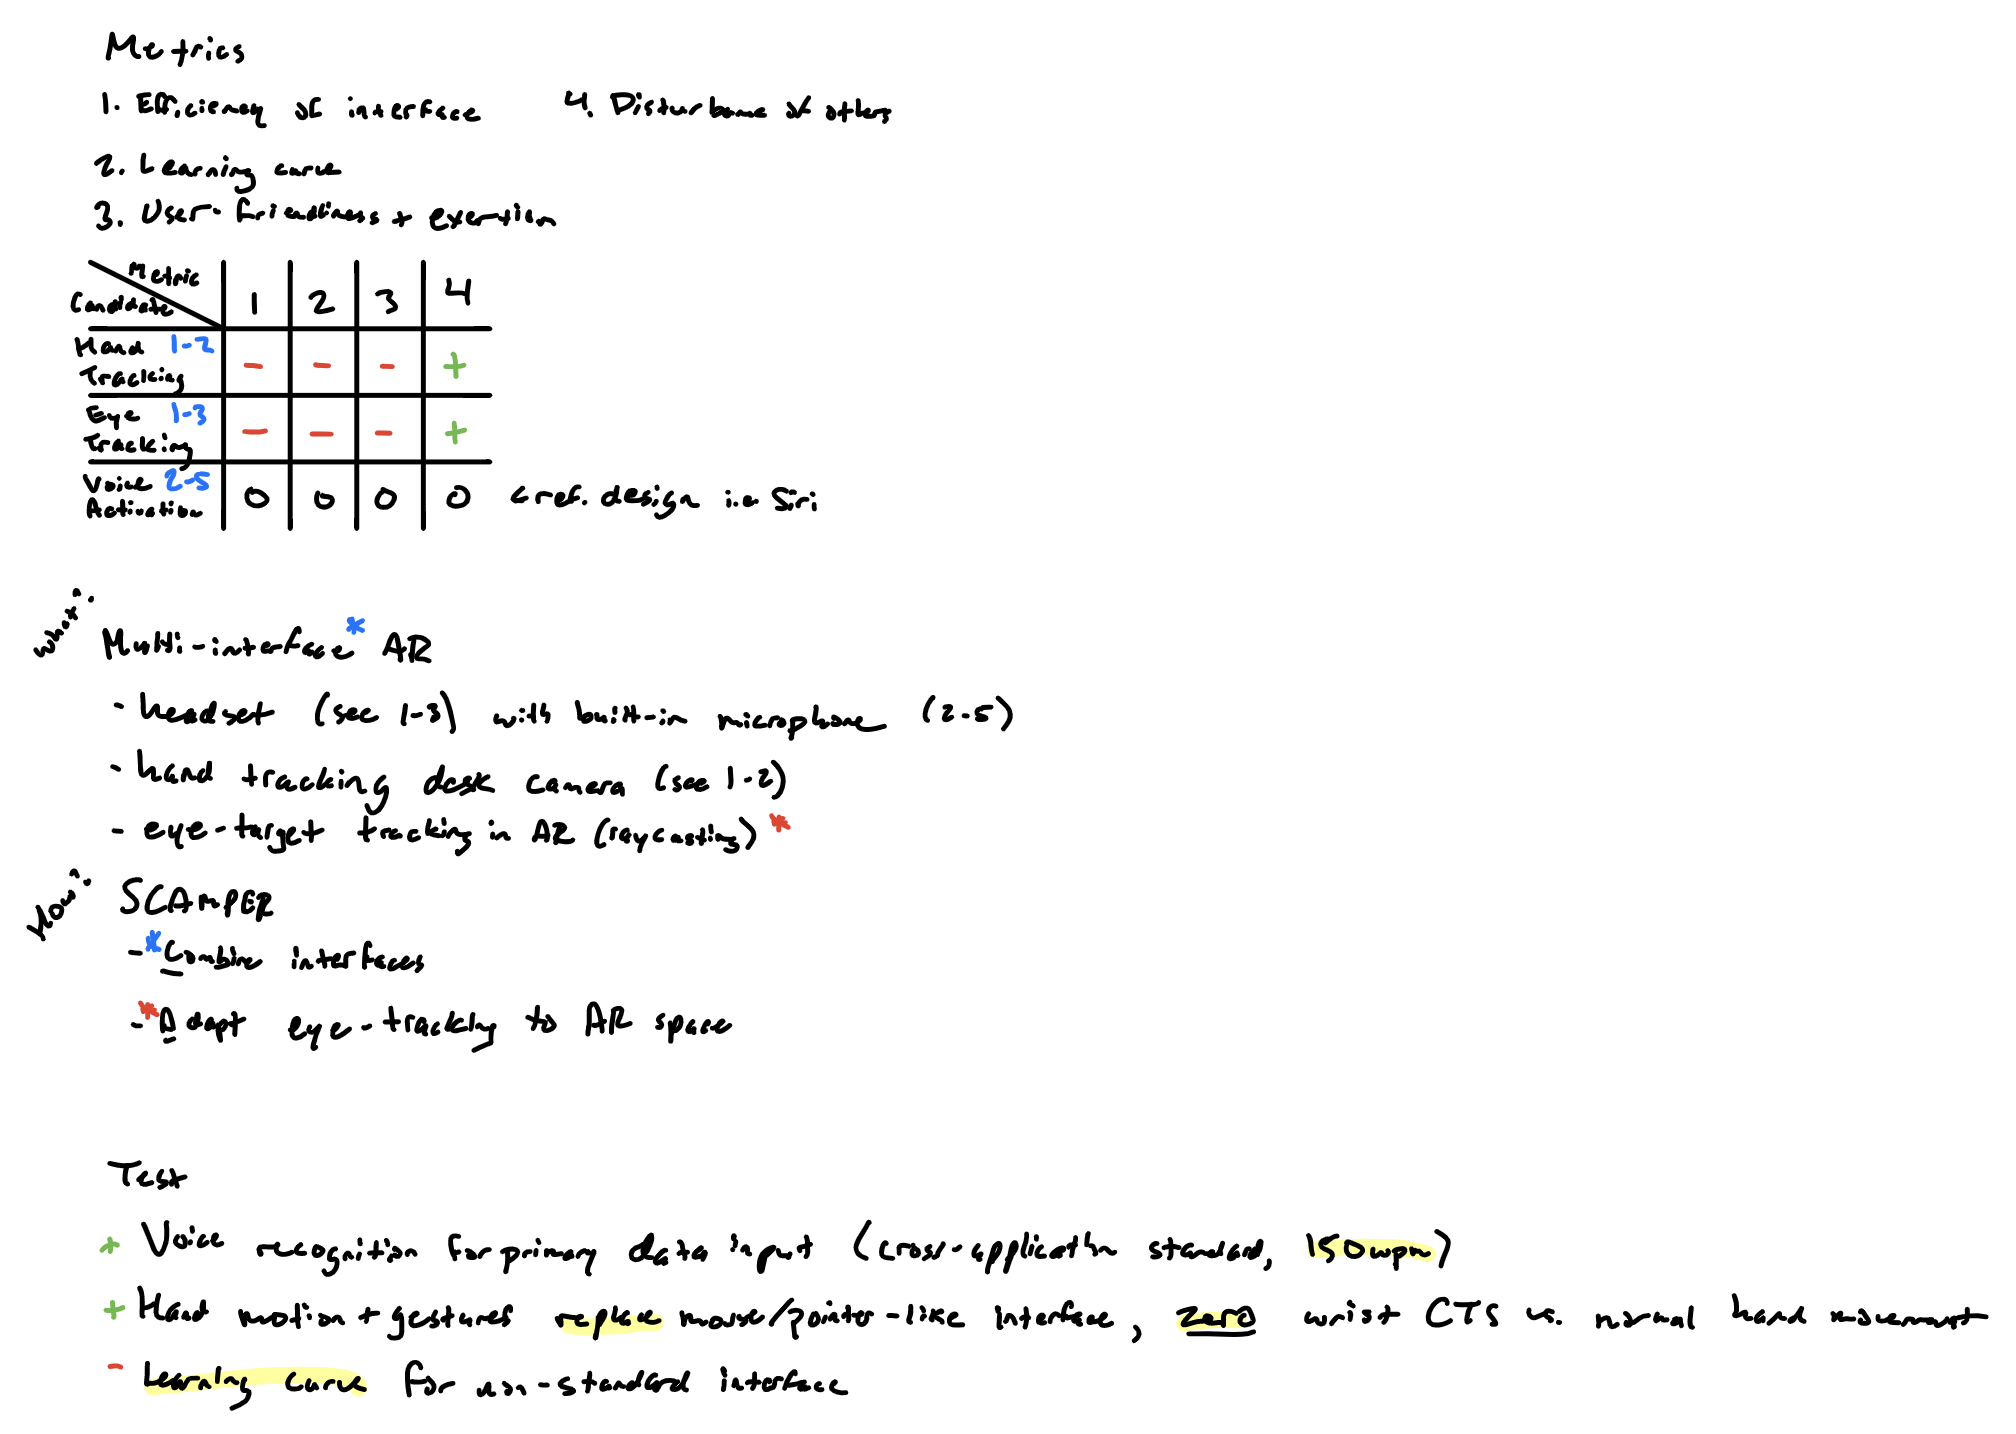
\includegraphics[width=\textwidth/2]{images/algorithm.png}
    \hfill
    \caption{An extract from my converging sprint notes. Though slightly illegible, it shows the development of category metrics (top-left) and feature recombination (centre) \cite{designcrit}.}
\end{figure}

\subsection{Praxis II Control Flow Diagram}
When developing prototypes that are meant to enact a certain process (“process 
prototypes”), it is often useful to lay out the process before any development 
occurs. This is especially true for technological prototypes, like programs. 
Starting from the most top-level “vision” of the prototype (some input produces 
some output) and breaking that down to the low-level “pseudocode” makes 
prototyping complex systems far easier. In essence, it is a framing process that
leads directly to development, which is extremely useful in practice.

\begin{figure}[h]
    \centering
    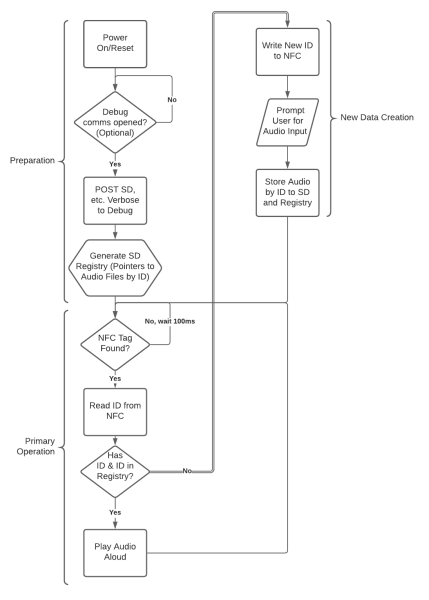
\includegraphics[width=\textwidth/2]{images/control.png}
    \hfill
    \caption{Control flow diagram prototype developed during Praxis II \cite{controlflow}.}
\end{figure}

\subsection{Praxis II Hardware Prototype and One-Pager}
As mentioned in the position section, I have a certain bias towards technical 
prototypes due to my interest in the field and past experience. However, I 
find there is a huge amount of payoff in developing a genuinely applicable 
prototype that could legitimately be used to solve the problem (call it a 
“coarse solution”) as compared to other prototypes (you know the ones, the 
cardboard-and-duct-tape ones). If I am able to develop a real solution, it 
feels like I’ve actually solved the problem and completed the engineering 
design process, as opposed to in Praxis I, where sprints were disjointed and 
never used the same topic twice.

The one-pager was also very useful, as it allowed the less technically-inclinded
members of my Praxis II team to gain a good understanding of how the device worked
from a functional standpoint. It also served as some pretty solid eye candy.

\begin{figure}[h]
    \centering
    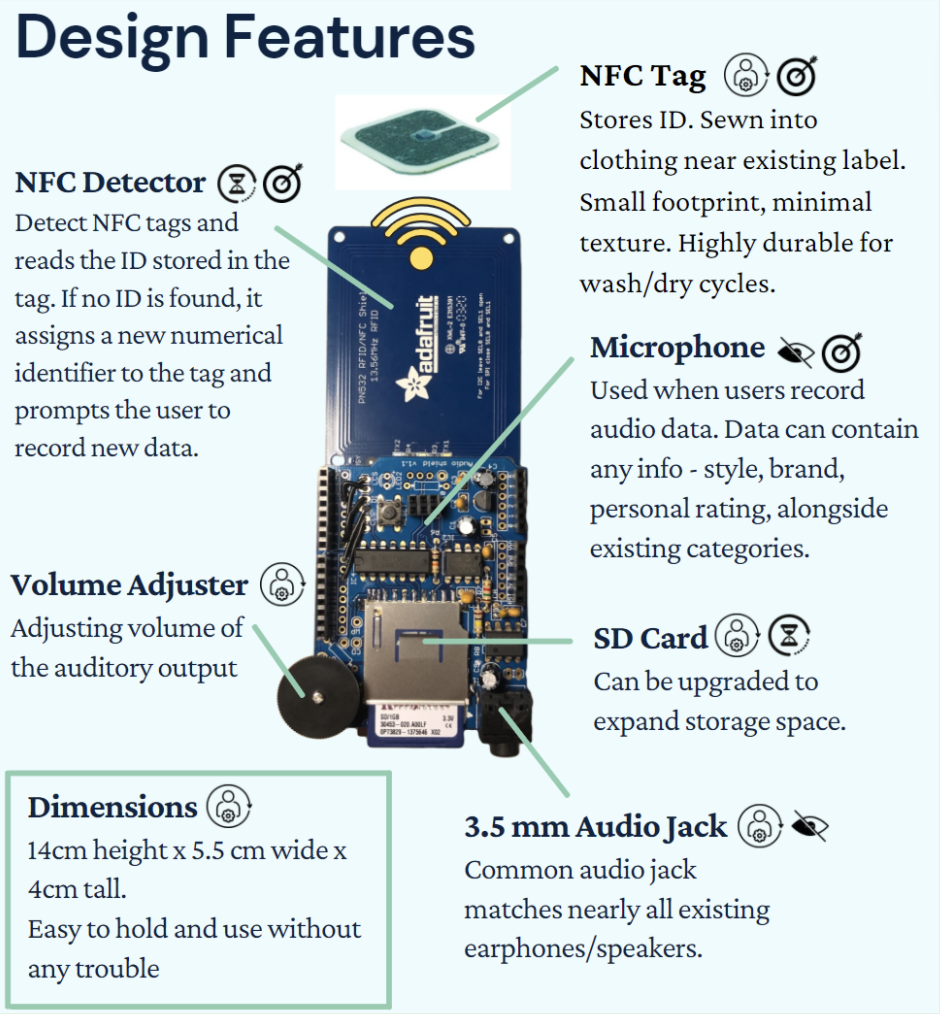
\includegraphics[width=\textwidth/2]{images/hardware.png}
    \hfill
    \caption{An extract from the one-pager (showing the hardware layout diagram) developed during Praxis II \cite{hardware}.}
\end{figure}

\pagebreak

\section{Process}
The way an opportunity is handled (where framing starts, how diverging/converging 
start) depend on the scope of the “problem statement” interpreted from the 
stakeholder’s lived experience. This process is largely derived from the 
parameter optimization approach, and incorporates the category genetic algorithm, 
both derived from what I learned in Praxis I.

\begin{figure}[h]
    \centering
    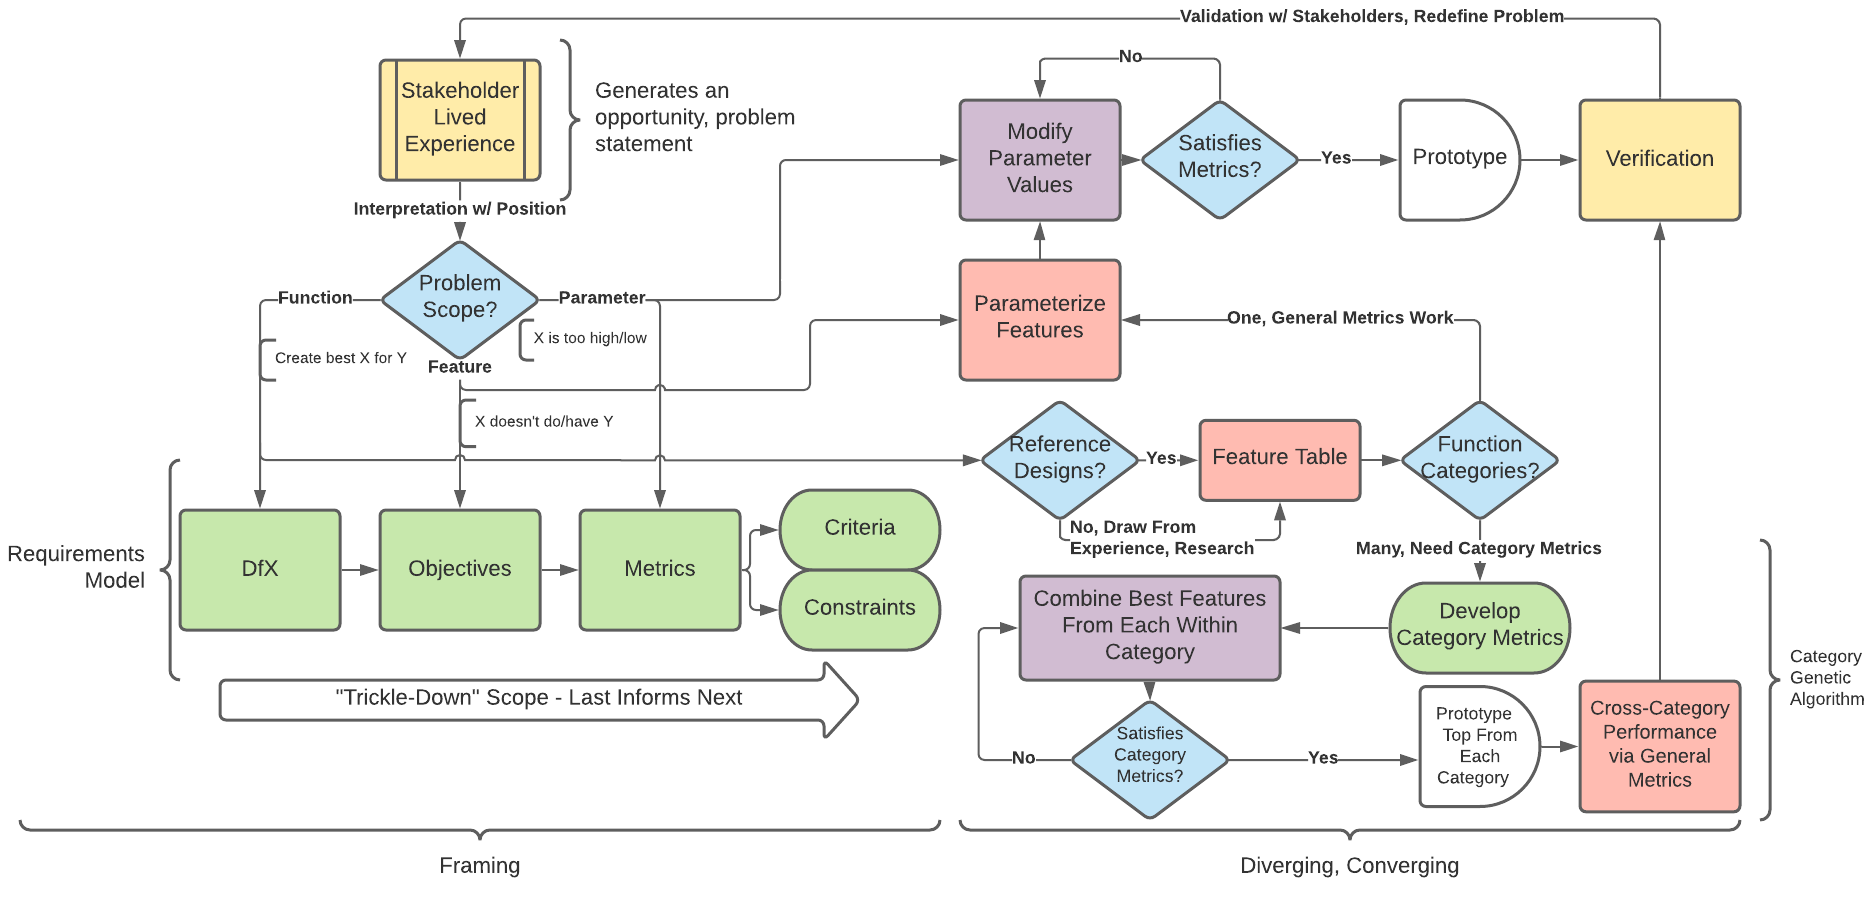
\includegraphics[width=\textwidth]{images/process.png}
    \hfill
\end{figure}

\pagebreak
\section{Tools, Models, and Frameworks}

All tools here are taken from the list "27 Creativity and Innovation Techniques Explained" provided on Quercus by the Praxis Teaching Team. You might notice that these are all converging and diverging tools - you would be correct. However, Framing comes very intuitive to me - I in fact don't recall using any framing tools beyond October, and their inclusion would be both counterproductive and tantamount to dishonesty.

\subsection{Attribute Listing}

After framing the problem down to the metric scope, the desired functions (and thus features)
of successful candidate designs can be listed. In this context, they are called attributes, and
parameters are built directly off of these: parameters control the "level" (more or less) of an attribute's
contribution to the ultimate design.

\begin{figure}[h]
    \centering
    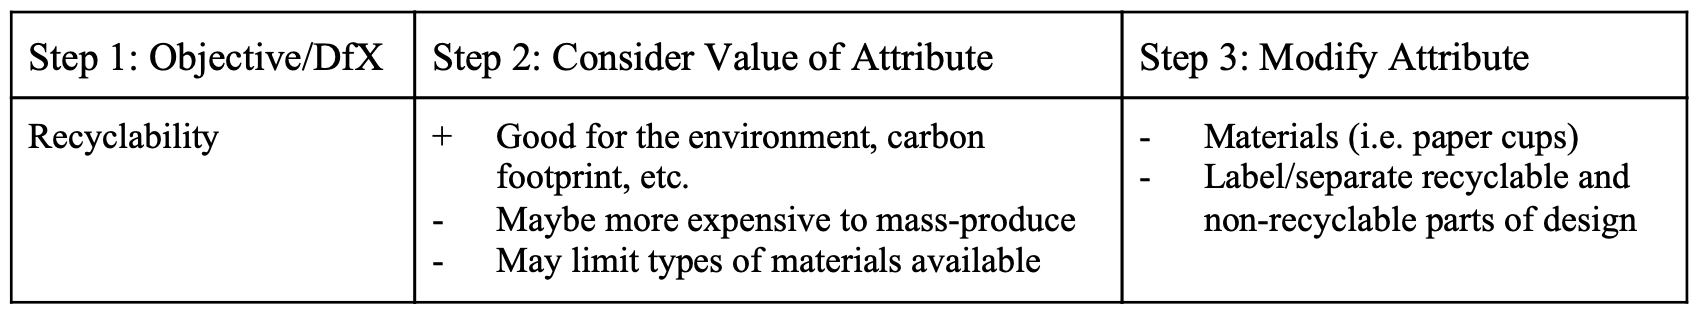
\includegraphics[width=\textwidth/2]{images/attributelisting.png}
    \hfill
    \caption{An example of attribute listing performed in the Praxis I diverging sprint \cite{candidatestools}.}
\end{figure}

By using a “first principles” approach to divergence based solely on the requirements model (as opposed 
to abstract brainstorming), my teams were able to explore the entire breadth of the opportunity. However, 
this tool also has the potential to be restrictive. For group members who might prefer abstract imagination, their 
ideas did not necessarily fit this model.

The straightforwardness and linearity of this tool allows high efficiency during the 
diverging process. There is also an increased sense of accomplishment, more so than when using 
other, less straightforward tools.

This tool is particularly useful at the start of diverging, as it helps to lay out the basis 
for a set of potential candidate designs. You can then adapt and branch off in order to develop 
more unique and imaginative ideas.

\subsection{Reverse Brainstorming}

The goal of reverse brainstorming is to change how a problem statement is worded from how it can be 
solved to how it can be caused. After different ways to cause the problem are identified, design 
functions that address each cause are proposed and potential features combined in order to target multiple factors 
in one candidate design.

\begin{figure}[h]
    \centering
    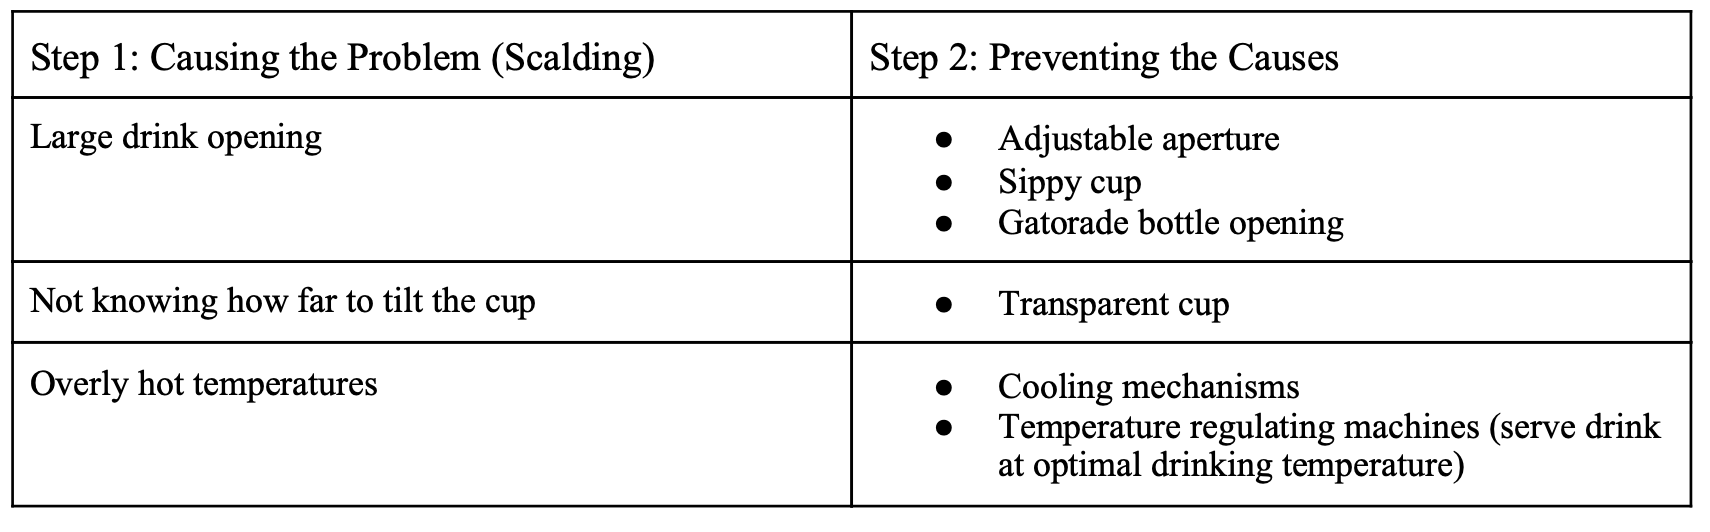
\includegraphics[width=\textwidth/2]{images/reversebrainstorm.png}
    \hfill
    \caption{An example of reverse brainstorming performed in the Praxis I diverging sprint \cite{candidatestools}.}
\end{figure}

Overall, reverse brainstorming is a helpful tool to use after doing some initial brainstorming, specifically 
in situations where the scope of an opportunity may stifle creativity or lead to anchoring. Reverse 
brainstorming is also useful for organizing candidate designs based on their function and for combining 
features of different candidate designs to target a variety of contributing factors related to the opportunity. 
Reverse brainstorming is also useful to expand scope by realize that there are many 
other factors that might be contributing to the problem, other than those initially identified during framing.
\pagebreak

\subsection{Pugh Chart}

Pugh Charts are particularly useful for recombination of successful features. The simple "better vs. worse" approach
to comparison allows for quick development (as opposed to assigning values and complex equations of "fit"), and also
lets you see which specific metrics are being met and by which features.

\begin{figure}[h]
    \centering
    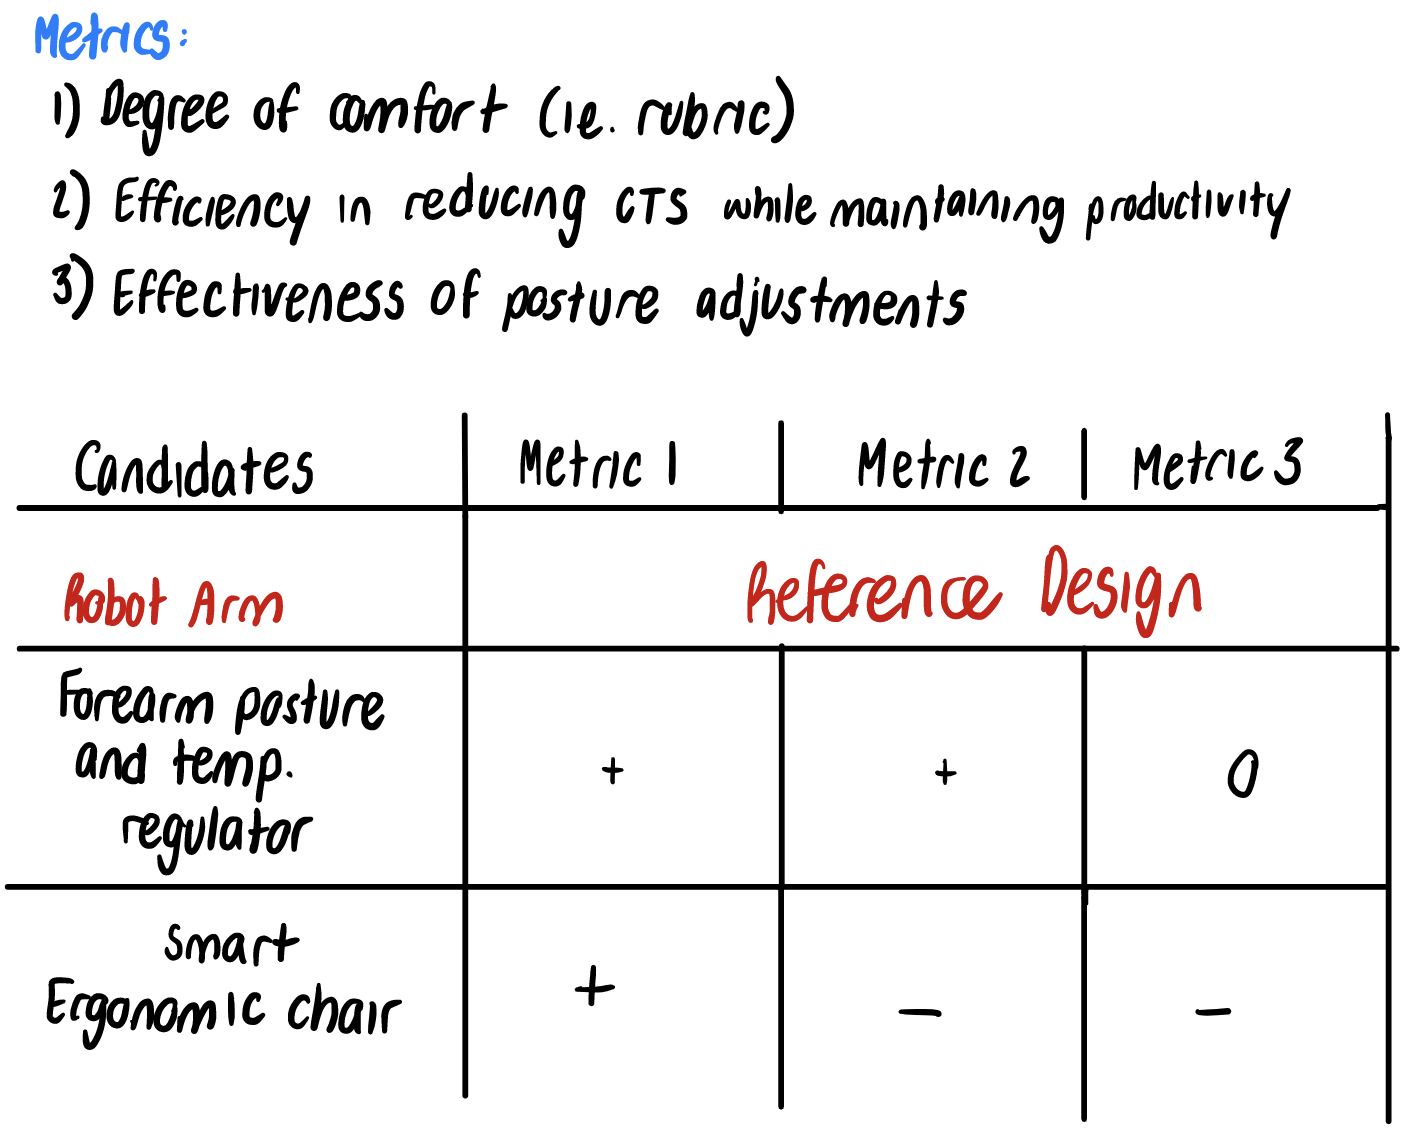
\includegraphics[width=\textwidth/2]{images/pughchart.png}
    \hfill
    \caption{An example of a Pugh Chart developed by one of my teammates during the Praxis I converging sprint \cite{designcrit}.}
\end{figure}

\pagebreak

\subsection{MORPH Chart}

MORPH charts allow for quick recombination of successful features into new designs in 5 different ways. This is especially important during the
converging-rediverging stage, as upon first analysis, it may appear that some designs are not feasible. However, this is often not the case;
some features may be advantageous to be incorporated into the final design.

\begin{figure}[h]
    \centering
    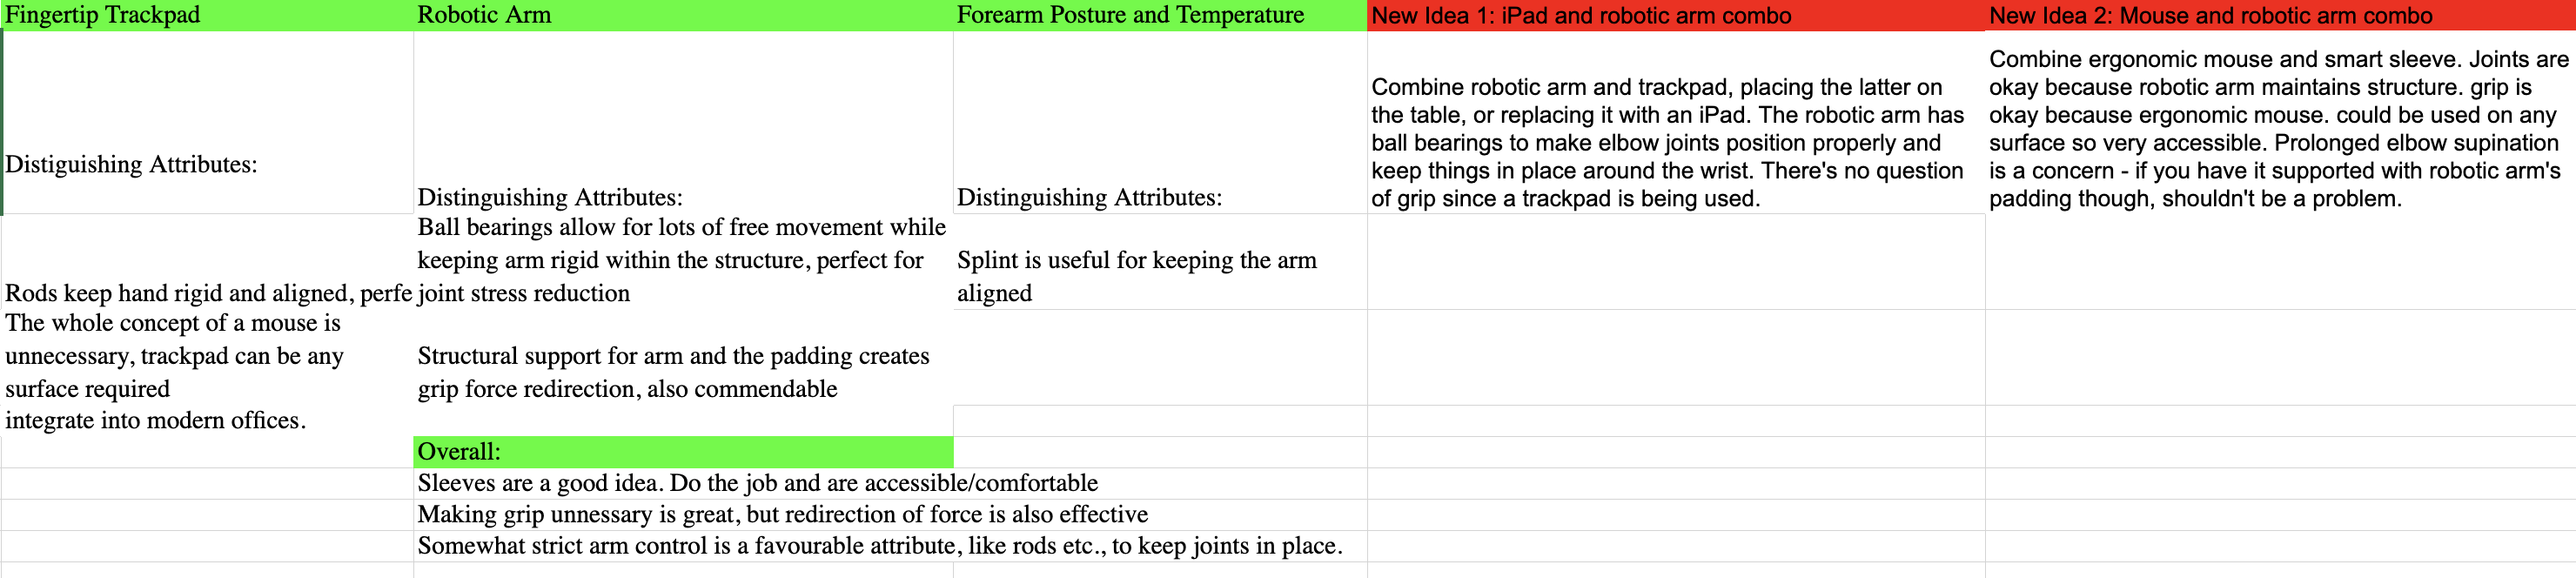
\includegraphics[width=\textwidth]{images/morphresults.png}
    \hfill
    \caption{The results of the usage of an adapted MORPH chart by one of my teammates during the Praxis I converging sprint \cite{designcrit}.}
\end{figure}

\pagebreak

\bibliographystyle{IEEEtran}

\bibliography{references}

\end{document}